\chapter{Cross-Language Experience for Current Cooperative Games}

 To understand how language barrier affects the cooperative experience for current games, we conducted a 12-person user study where half the participants shared common languages and half did not. 

\section{Study Design}

We recruited 3 Japanese speakers and 9 Taiwanese speakers, and confirmed that none of the Taiwanese speakers understood Japanese and vice versa. 3 pairs of the participants did not have a common language (Japanese-Taiwanese) and 3 pairs did (Taiwanese).

We selected 3 popular cooperative games currently on the market that had distinct gameplay and cooperation needs. Also, all three games supported real-time voice chat. 
\begin{enumerate}
    \item Rocketbirds - Hardboiled Chicken: a cooperative action game, in which players shoot enemies with different weapons.
    
    \item Portal 2: a cooperative puzzle game, in which players can create portals that teleport players and must use them intelligently to solve the puzzles.
    
    \item Monaco: a cooperative stealth game, in which players can evade guards, collect coins, and escape.
\end{enumerate}

In order to simulate cooperative gameplay over the Internet, pairs of players were placed in two different rooms and used headsets to communicate with each other. Participants played each of the three games for 30 minutes, and filled out an eSFQ\cite{eSFQ} questionnaire after each game. We also conducted open-ended interviews to understand their gaming experience at the end of the sessions. 



\section{Results}

eSFQ\cite{eSFQ} has been widely used for rapid assessment of game experience. Players are asked to provide Likert-scale ratings (on a scale of 1 to 5) and to select multiple keywords to describe aspects of their experience. 
For this study, we focus on the fun/enjoyment ratings and the frustrating co-experience. 

\begin{figure}[!t]
\centering
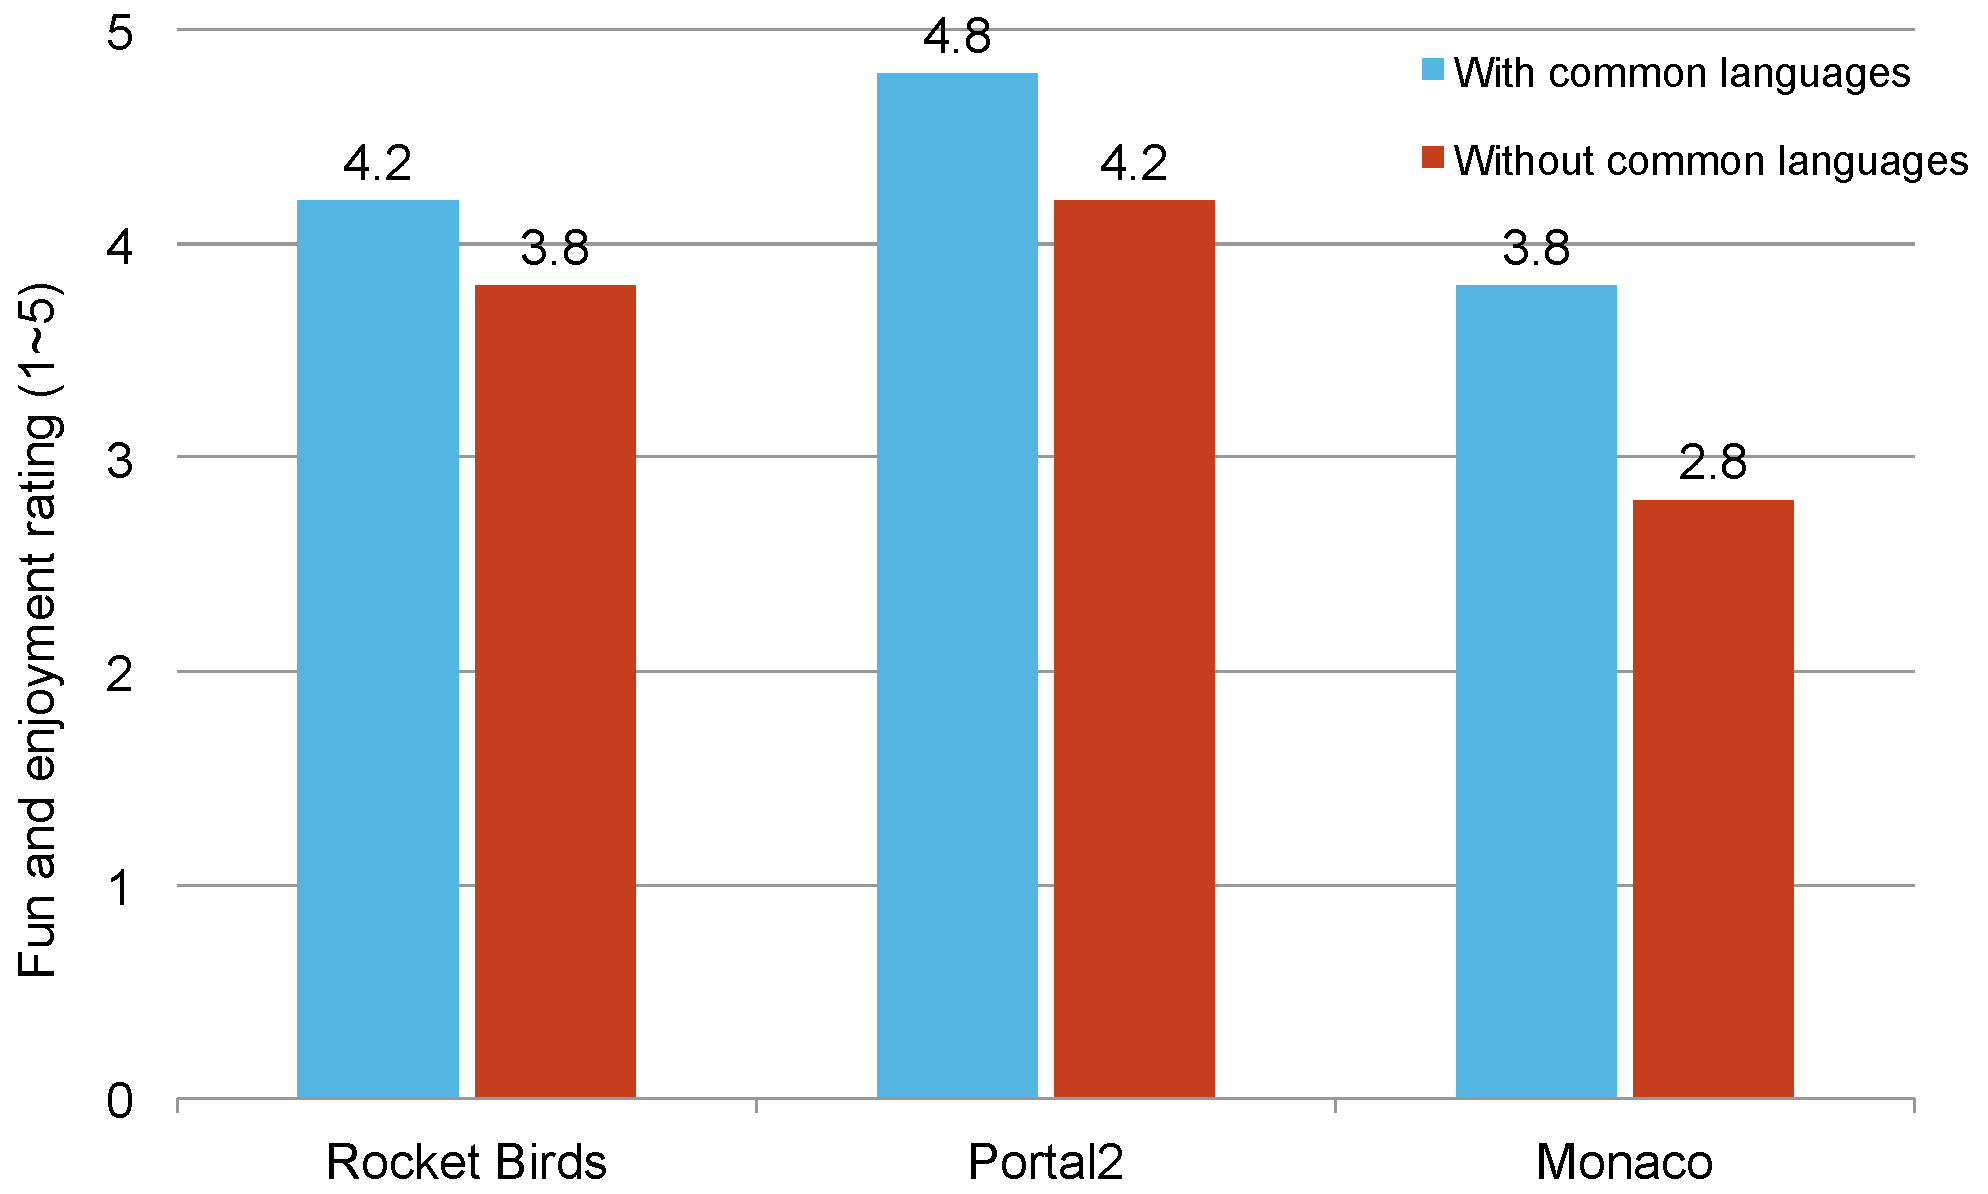
\includegraphics[width=0.9\columnwidth]{Figures/PS_FunAndEnj.pdf}
\caption{The eSFQ Fun and Enjoyment rating (on a scale of 1 to 5) of three cooperative games for players \textit{with} and \textit{without} common languages.}
\label{fig:PS_FunAndEnj}
\end{figure}


\begin{figure}[!t]
\centering
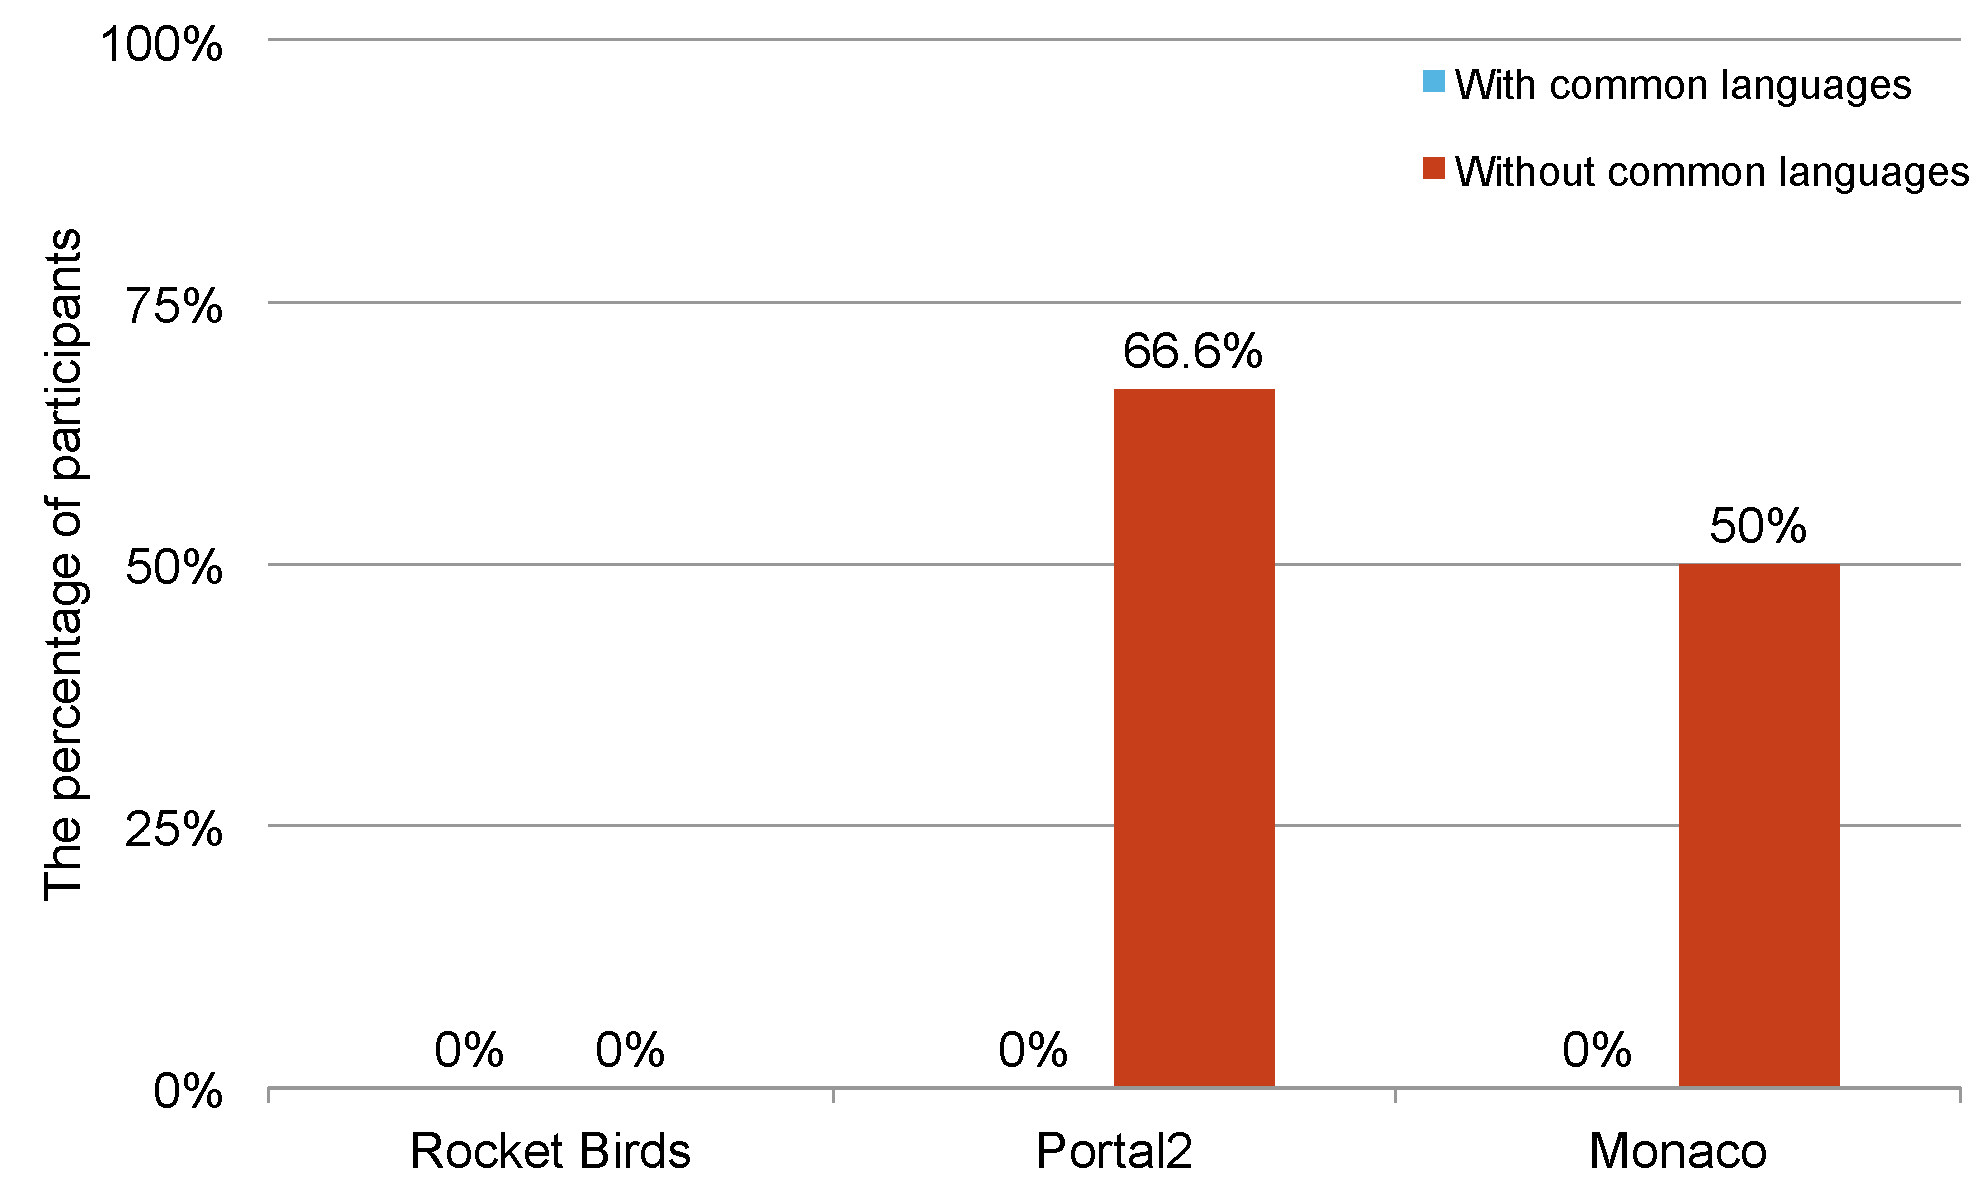
\includegraphics[width=0.9\columnwidth]{Figures/PS_Frus.pdf}
\caption{The eSFQ Frustration index, which is the percentage of players who reported a frustrating experience, of three cooperative games for players \textit{with} and \textit{without} common languages.}
\label{fig:PS_Frus}
\end{figure}


Figure~\ref{fig:PS_FunAndEnj}, shows the average eSFQ Fun and Enjoyment rating for each game, for players \textit{with} and \textit{without} common languages. 
A rating of 5 is the highest level of fun and means ``Yeah, fun'', and a rating of 1 is the lowest level of fun and means ``Yawn, boring''.
The rating was lower for all three games when the players did not have common languages. Overall, the Fun and Enjoyment rating was 3.6 vs 4.3 for players without common languages compared to those who could communicate using a common spoken language.

Figure~\ref{fig:PS_Frus} shows the eSFQ Frustration index, which is the percentage of players who reported the experience as frustrating, for players \textit{with} and \textit{without} common languages.
For two out of the three games, Portal 2 and Monaco, frustration is significantly higher for players without common languages than those who did. In fact, none of the players with a common spoken languages reported any of the games as frustrating. 


\section{Discussion}

The Rocketbirds' gameplay mainly consists of dodging and shooting, and required the least communication outside the game. As player P5 commented (shown in Table 1): ``We couldn't talk to each other, but communicated through moves and jumps.'' 
None of the players reported Rocketbirds as frustrating, and language barriers had the least effect on its fun and enjoyment rating as well.

Portal 2 was reported as the most frustrating by players without common languages. Portal 2's primary gameplay is to solve complex puzzles, which requires precise collaboration between the two partners. As some of the players mentioned: ``I couldn't tell what my partner was trying to do without talking to each other.''(P5), and ``It was tiring because it was hard to express my ideas.'' (P4).

Monaco's gameplay allowed a single player to solve a challenge, although cooperation would make it significantly easier. Player P4 mentioned: ``I didn't know where the exit was, and my partner couldn't tell me.'', yet P9 stated:  ``This game is simple. We didn't really need any communication with each other.''.



\vspace{4ex}
\begin{table}[htbp]
    \centering
    \begin{tabular}{|p{100pt}|p{250pt}|}
        \hline
            Game & Feedback from Players without Common Languages\\
        \hline
        	Rocketbirds & \begin{itemize}
	 	 \item ``Although it was slower without talking, the challenges could still 
    	be beaten with patience.''(P2)
    	\item ``We couldn't talk to each other, but communicated through moves and jumps.''(P5)
	  	\end{itemize}
    	\\
        \hline
            Portal 2 & 
    	\begin{itemize}
    	\item ``It was tiring because it was hard to express my ideas.''(P4)
    	\item ``I couldn't tell what my partner was trying to do without talking to each other.''(P5)
    	\end{itemize}
    	\\
        \hline
        Monaco & 
    	\begin{itemize}
    	\item ``I didn't know where the exit was, and my partner couldn't tell me.''(P4)
    	\item ``This game is simple. We didn't really need any communication with each other.''(P9)
    	\end{itemize}
    	\\
    	\hline
    \end{tabular}
    \caption{Interview comments by players without common languages.}
  	\label{tab:table1}
\end{table}


% \begin{table}[!h]
%   \centering
%   \begin{tabular}{
%   !{\vrule width2pt}c
%   !{\vrule width2pt}p{0.7\columnwidth}
%   !{\vrule width2pt}c}
%     \hline
%     \centering\tabhead{Game} &
%     \multicolumn{1}{p{0.7\columnwidth}!{\vrule width2pt}}{\centering\tabhead{Feedback from Players without Common Languages}} \\
%     \hline
%     Rocketbirds & 
%     \begin{itemize}
% 	  \item ``Although it was slower without talking, the challenges could still 
%     be beaten with patience.''(P2)
%     \item ``We couldn't talk to each other, but communicated through moves and jumps.''(P5)
% 	  \end{itemize}
%     \\
%     \hline
%     Portal 2 & 
%     \begin{itemize}
%     \item ``It was tiring because it was hard to express my ideas.''(P4)
%     \item ``I couldn't tell what my partner was trying to do without talking to each other.''(P5)
%     \end{itemize}
%     \\
%     \hline
%     Monaco & 
%     \begin{itemize}
%     \item ``I didn't know where the exit was, and my partner couldn't tell me.''(P4)
%     \item ``This game is simple. We didn't really need any communication with each other.''(P9)
%     \end{itemize}
%     \\
%     \hline
%   \end{tabular}
%   \caption{Interview comments by players without common languages.}
%   \label{tab:table1}
% \end{table}
